\chapter{Wind Turbine Monitoring} \label{s:wt_monitoring}

In this chapter a brief overview of which components make up a wind turbine will be given, and how a wind turbine functions. 
Further, the different machine learning techniques enountered will be shown, and the theory behind the most popular models will be explained. The chapter will end with a discussen about the advantages of the different models in relation to what kind of data one has available.

\section{Wind turbine Components}

\begin{figure}[h]
    \begin{center}
    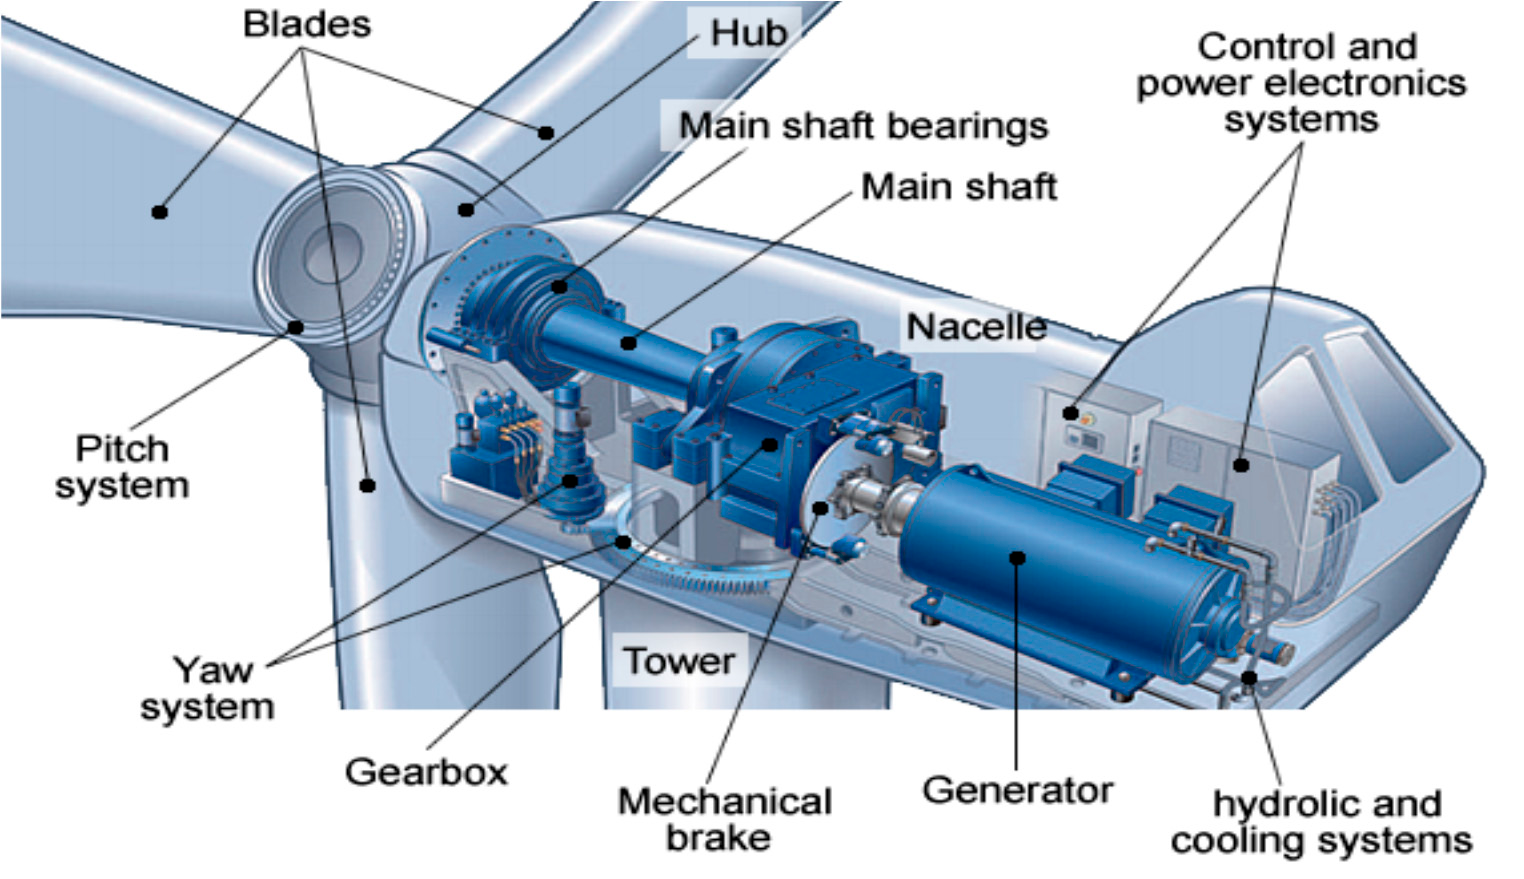
\includegraphics[width=0.8\textwidth]{wind_turbine/wt_parts.png}
    \end{center}
    \caption{Illustration of the different parts of a wind turbine, taken from \textcite{adv_meth_for_wt_cond_monit_rev}}
    \label{fig:wt_parts}
\end{figure}

Figure \ref{fig:wt_parts} shows the main parts of a wind turbine which includes the rotor (blades and hub), shafts, gearbox and generator. 
Simplified a wind turbine works by wind pushing the blades, generating torque that makes the hub rotate. 
The hub is connected to the gearboxjkk through the main shaft. 
The gearbox then gears down the torque and gears up the rotational speed to a level that the generator can use to induce current, that goes to a station that transforms the voltage to a level that can be used in the electrical grid. 

\section{Sensors and Data Acquisition}

Information about a wind turbine can come from many sources, it can come from external sources such as images from a camera, or from internal sensors measuring operational data. 
The collective term for systems measuring operational data is supervisory control and data acquisition (SCADA) systems. 
To choose what algorithm to use, or what model to use, one must first consider what data one has available. 
From the literature considered, these where the most used forms of data used as input for the model:

\begin{itemize}
    \item Vibration measurement  
    \item Acoustic emission monitoring 
    \item Temperature measurement 
    \item Power signal measurement 
    \item Oil debris monitoring 
    \item Strain monitoring 
    \item Optical fiber monitoring 
    \item Ultrasonic testing 
    \item Image analysis
\end{itemize}

Analysis of vibration signals is the most common form of condition monitoring used in industry for any form of rotating equipment \cite{wt_bearing_cm_review}. 
By measuring the acoustic emission generated by a component of a wind turbine, one can estimate how much damage it has sustained. 
The temperature of components in a wind turbine is closely correlated with the health of the component, and is therefore used often in condition monitoring applications \cite{DBN_chicken_swarm_optim}. 
The power signal can also say a lot about how wind turbine is performing, specifically the wind speed - power curve. 
When monitoring the debris in the oil of a wind turbine gearbox one is analysing the size, type and number of wear particles present in the lubricant, as they can indicate the degree of damage in the gearbox \cite{cm_rnn_lstm}. 
Strain monitoring, optical fiber monitoring, ultrasonic testing, and image analysis are all used to detect structural damage in different components of the wind turbine, usually the blades \cite{lin_and_non_lin_feat_for_ice_detection_on_blades, image_based_surface_damage_detection_DL_drone_inspection,image_based_YOLO_YSODA, dirt_n_mud_detection_using_guided_waves,blade_defect_detection_imaging_array, unsupervised_AD_blade_damage_deep_features_images}, or tower \cite{wt_cm_rev_new_trends_chal_2014}. 
However, the most common approach was to use a combination of multiple sensor-values to make predictions about the condition about the wind turbine.

\section{Machine Learning Techniques}
A machine learning is a subset of artificial intelligence. 
Machine learning models extract rules from data, which can then be applied to classify, or estimate components of another dataset. 
Machine learning algorithms are formally divided into \textit{supervised learning}, \textit{unsupervised learning} and \textit{semi-supervised learning}. 
Supervised learning models require labelled datasets to extract information from the dataset, and are usually used to perform classification tasks, or to estimate a variable that is considered dependent on the input variables (regression). 
Unsupervised learning algorithms do not require labelled datasets. 
Semi-supervised learning uses a combination of labelled and unlabelled datasets. 
The different machine learning models encountered are split into regression-based models, supervised classification-based models and unsupervised classification-based models. 


\subsection{Feature Extraction}
There are two central problems in condition monitoring that can be solved by feature extraction and selection. 
The first is the sheer volume of information being produced. 
A wind turbine with only 20 sensors, sampled at 100 Hz will produce 170 MB of information per day. 
Feature selection is used here to reduce the number of features to only those relevant for condition monitoring. 
The second problem is that for systems using only one signal such as vibration, there are many components that are superposed to create the measured signal, and noise is present. 
Feature extraction is used to separate the interesting components from each other, and cancel the noise. 
For some machine learning models feature extraction is not a neccesary preprocessing step. 
For others, careful thought must be given as to how to extract features. 
Table \ref{tab:feat_ext_wt} shows the most frequent methods found in the articles. \bigskip

\begin{table*}
    \centering
    \ra{1.3}
    \begin{tabular}{p{0.31\textwidth}p{0.3\textwidth}}
        \toprule
        Extraction method                   & Articles \\
        \midrule
        ARMA models                         & \cite{ml_cm_wt_blade_ARMA_2018, fault_detection_and_isolation_using_classifier_fusion, lin_and_non_lin_feat_for_ice_detection_on_blades, dirt_n_mud_detection_using_guided_waves, vibration_ARMA_decision_tree_cm_wt} \\
        Discrete Wavelet Transform (DWT)    & \cite{fault_detection_and_isolation_using_classifier_fusion, image_texture_analysis_FD_wt, vibration_acustic_decision_tree_SVM_gearbox, integrated_cm_bearing_fault_wt_gearbox} \\
        Principal Component analysis (PCA)  & \cite{lin_and_non_lin_feat_for_ice_detection_on_blades, multiway_PCA_multivar_inference_cm_wt, dirt_n_mud_detection_using_guided_waves, integrated_cm_bearing_fault_wt_gearbox, unsupervised_AD_blade_damage_deep_features_images, online_fd_using_PCA_different_operating_zones, fault_detect_PARAFAC_k_means}\\
        Basic signal statistics             & \cite{blade_damage_detection_sup_ml_alg, integrated_cm_bearing_fault_wt_gearbox, roller_bearings_cm_fisher_score_and_permutation_entropy} \\
        \bottomrule
    \end{tabular}
    \caption{Feature extraction methods}
    \label{tab:feat_ext_wt}
\end{table*}

The DWT is a method used for decomposing time-dependent signals.
Compared to the discrete Fourier transform (DFT) the DWT can capture time-dependent and frequency-dependent information of a time series, which makes it more suitable for non-stationary signals. 
However, the DFT is also used \cite{fault_detection_and_isolation_using_classifier_fusion, blade_damage_detection_sup_ml_alg}. 
Basic signal statistics refers to values easy to calculate over a fixed window size, such as the root-mean-square (RMS) value and the min/max value 
ARMA models are frequently used for time signal analysis, and will be expanded upon in section \ref{sec:ts_models}. 
PCA is an unsupervised machine learning form used in multivariate systems. 
It produces the linear combinations of variables that has the highest variance, also called the \textit{principal components}.
PCA, and generalizations of PCA is also a valuable tool for dimensionality reduction, and will also be expanded upon, in section \ref{sec:ts_models}. 
% EXPLAINING MODELS
Before going into which machine learning models have been used for condition monitoring, an extended explanation will be given of some of the more complex, and most used machine learning models: Artificial neural networks (ANNs), networks of restricted Boltzman machines (RBMs) and support vector machines (SVMs). 
A brief explanation will be given about the other models encountered as well. 

\newpage
\subsubsection*{Artificial Neural Networks}
Figure \ref{fig:perc_nn} $(a)$ depicts the building blocks of an ANN, the perceptron. 
The perceptron is a model of an artificial neuron, it takes in $n$ inputs, performs a weighted sum of the inputs and a bias $b$, and sends the sum through an objective function. 
Originally the objective functions were just threshold functions returning 1 if the sum was above the threshold, and 0 if the sum is below the threshold. 
When one started using multiple layers of perceptrons as ANNs, other objective functions where introduced including $tanh$, $sigmoid$ and the \textit{recitfied linear unit}. 
The perceptron is only able to perform binary classification on points that are linearly separable. 
However, by combining multiple layers of perceptrons into networks, training the network with the backpropagation algorithm and by intruducing non-linear objective functions ANNs are able to capture complex non-linear relationships.
A simple ANN is depicted in figure \ref{fig:perc_nn} $(b)$. 
The first layer in an ANN is called the input layer, the last layer is called the output layer and all the layers inbetween are called hidden layers.
ANNs using special perceptrons with ''memory'' also exist, and are called recurrent neural networks (RNNs). 
Some ANNs use special layers that only perform wieghted sums with the closest set of neurons from the previous layer, such networks are called convolutional neural networks (CNNs).
If one designs an ANN to have as many perceptrons in the output layer as in the input they can be used as a generative model to recreate the input, this is what is known as an autoencoder.

\begin{figure}
\begin{center}
    \tikzstyle{init} = [pin edge={to-,thin,black}]
\tikzstyle{circ} = [circle, minimum size=1cm, text centered, draw=black, fill=blue!20]
\tikzstyle{arrow} = [thin,->,>=stealth]

\tikzstyle{perc_in} = [circle, minimum size=1mm, text centered, draw=black, fill=blue!20]
\tikzstyle{perc_ou} = [circle, minimum size=1mm, text centered, draw=black, fill=red!20]
\tikzstyle{perc_hi} = [circle, minimum size=1mm, text centered, draw=black, fill=green!20]

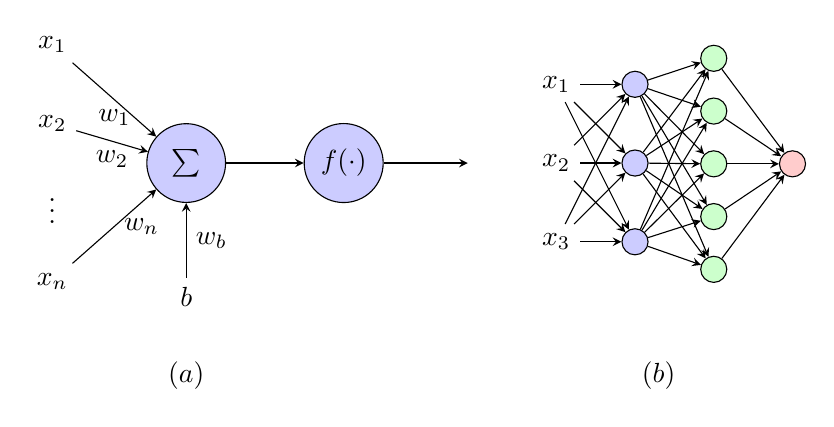
\begin{tikzpicture}
% Perceptron
\node (x1) [init] {$x_1$};
\node (x2) [init, below of=x1] {$x_2$};
\node (vdots) [init, below of=x2] {$\vdots$};
\node (xn) [init, below of=vdots] {$x_n$};

\node (sum) [circ, right of=x2, xshift=0.7cm, yshift=-5mm] {$\sum$};
\node (b) [init, below of=sum, yshift=-0.7cm] {$b$};
\node (obj) [circ, right of=sum, xshift=1cm] {$f(\cdot)$};
\node (output) [init, right of=obj, xshift=0.7cm] {};

\draw [arrow] (x1) --node[anchor=north] {$w_1$} (sum);
\draw [arrow] (x2) --node[anchor=north] {$w_2$} (sum);
\draw [arrow] (xn) --node[anchor=west] {$w_n$} (sum);
\draw [arrow] (b) --node[anchor=west] {$w_b$} (sum);
\draw [arrow] (sum) -- (obj);
\draw [arrow] (obj) -- (output);

% ANN
\node (i2) [init, right of=output] {$x_2$};
\node (i1) [init,, above of=i2] {$x_1$};
\node (i3) [init, below of=i2] {$x_3$};

\node (in0) [perc_in, right of=i1] {};
\node (in1) [perc_in, below of=in0] {};
\node (in2) [perc_in, below of=in1] {};

\node (hi0) [perc_hi, right of=in0, yshift=3.3mm] {};
\node (hi1) [perc_hi, below of=hi0, yshift=3.3mm] {};
\node (hi2) [perc_hi, below of=hi1, yshift=3.3mm] {};
\node (hi3) [perc_hi, below of=hi2, yshift=3.3mm] {};
\node (hi4) [perc_hi, below of=hi3, yshift=3.3mm] {};

\node (ou0) [perc_ou, right of=hi2] {};

\draw [arrow] (i1) -- (in0);
\draw [arrow] (i1) -- (in1);
\draw [arrow] (i1) -- (in2);
\draw [arrow] (i2) -- (in0);
\draw [arrow] (i2) -- (in1);
\draw [arrow] (i2) -- (in2);
\draw [arrow] (i3) -- (in0);
\draw [arrow] (i3) -- (in1);
\draw [arrow] (i3) -- (in2);

\draw [arrow] (in0) -- (hi0);
\draw [arrow] (in0) -- (hi1);
\draw [arrow] (in0) -- (hi2);
\draw [arrow] (in0) -- (hi3);
\draw [arrow] (in0) -- (hi4);
\draw [arrow] (in1) -- (hi0);
\draw [arrow] (in1) -- (hi1);
\draw [arrow] (in1) -- (hi2);
\draw [arrow] (in1) -- (hi3);
\draw [arrow] (in1) -- (hi4);
\draw [arrow] (in2) -- (hi0);
\draw [arrow] (in2) -- (hi1);
\draw [arrow] (in2) -- (hi2);
\draw [arrow] (in2) -- (hi3);
\draw [arrow] (in2) -- (hi4);

\draw [arrow] (hi0) -- (ou0);
\draw [arrow] (hi1) -- (ou0);
\draw [arrow] (hi2) -- (ou0);
\draw [arrow] (hi3) -- (ou0);
\draw [arrow] (hi4) -- (ou0);

\node (label_a) [init, below of=b] {$(a)$};
\node (label_a) [init, right of=label_a, xshift=5cm] {$(b)$};
\end{tikzpicture}
\end{center}
\caption{$(a)$ A Perceptron. $(b)$ Example of a simple ANN.} 
\label{fig:perc_nn}
\end{figure}

\subsubsection*{Support Vector Machines}
SVMs were originally implemented as a type of binary classifier that could classify linearly separable variables.
The SVM transforms input variables to a set of hyperplanes, which can be used both for classification and regression tasks \cite{svm_wikipedia}. 
However, by introducing kernel functions one became able to map the input data to a vector space where they are linearly separable.
Some example of kernel functions include: Linear kernal, radial basis function and sigmoid function. 

\subsubsection*{Restricted Boltzman Machines}
RBMs can be considered as a stochastic neural network with two layers, an input layer and a hidden layer \cite{DBN_chicken_swarm_optim}, note that they do not have an output layer. 
The defining difference between RBMs and ANNs is that ANNs are deterministic models, while the units that make up an RBM are inherently stochastic. 
RBMs alone are said to be generative models \cite{rbm_wikipedia}, like the autoencoder. 
If one combines multiple RBMs, such that the hidden layer of one RBM feeds in to the input layer of another, and combines this with a final output layer one has a deep belief network (BDN). 
DBNs can perform discriminative tasks such as classification and regression, and are not solely generative as the RBMs alone.

\subsubsection*{Other models}
Gaussian processes (GPs) are a probabilistic machine learning technique that can be used for regression, and classification tasks. 
Similar to SVMs they perform best when the relationship between the input variables and the target variable are linear, but by the use of kernels one can map the input variables to a hyperplane where the targets are linearly seperable. \cite{GP_book}
The defining diference are that GPs are probabilistic while SVMs are deterministic. 
K-nearest neighbors is a machine learning model that can be used for classification and for regression. 
When used for regression the target is predicted based on the points from the training set which are ''nearest'' in terms of input variable values \cite{high_freq_scada_perf_monit_sensitivity}.
Random forests (RF) when used for regression tasks randomly create regressors which each give a prediction of the target variable \cite{high_freq_scada_perf_monit_sensitivity}. 
Through the training process the model learns which regressors should have more weight in the final prediction. 

\subsection{Regression-based Models}
A frequent approach is to use a supervised learning model to capture the normal behaviour of a wind turbine, or wind turbine component, by predicting the value of one time dependent variable, or by recreating the input variables. 
Then the deviation between the prediction and the actual value is used to detect anomalous behaviour. 
If the system attempts to predict one variable this deviation is called the estimation error ($E_e$), if the system is intended to recreate the input the deviation is called the reconstruction error ($R_e$).
The input data used in this approach is most often SCADA data. 
What varies in these approaches is what machine learning model they use to model the wind turbine. 
Three curves in particular hold a lot of information about the performance of a wind turbine, namely the wind speed, active power curve; wind speed, rotor speed curve and wind speed, blade angle pitch curve. 
The majority of the regression based models used a subset of these curves as target variables \cite{perf_mon_of_wt_using_extreme_func_theory, GP_operational_curve_monitoring, high_freq_scada_perf_monit_sensitivity, abnormal_detection_scada_data_mining, improved_power_curve_monitoring_of_wt, SVR_blade_pitch_curve_cm, health_cond_model_nn_proportional_hazard_models}. 
Another popular approach is to attempt to forecast the temperature in the gearbox, or generator windings \cite{AD_and_fault_analysis_wt_DAE, health_cond_model_nn_proportional_hazard_models, detecting_malfunctions_wt_generator_bearings_generic_vs_specific_models, CBPM_ABPM_maintainance_model, wt_gearbox_bearing_temp_KS_CNN, DBN_chicken_swarm_optim}. 
As mentioned before temperature is closely correlated with the health of a component, but since temperature changes so slowly it is hard to use temperature monitoring alone for fault prediction \cite{wt_cm_rev_new_trends_chal_2014}. 
However, if one can make a model capture the complex sources of temperature change, the deviation between predicted temperature, and actual temperature could be used for fault prediction. 
Table \ref{tab:regression_ml_models} shows the typical machine learning models used for regression. 

\begin{table*}[h]
    \centering
    \ra{1.3}
    \begin{tabular}{p{0.45\textwidth}p{0.3\textwidth}}
        \toprule
        Machine learning model  & Articles \\
        \midrule
        ANNs                    & \cite{improved_power_curve_monitoring_of_wt, ANN_damage_detection_gearbox_wt, health_cond_model_nn_proportional_hazard_models, detecting_malfunctions_wt_generator_bearings_generic_vs_specific_models, CBPM_ABPM_maintainance_model, wt_gearbox_bearing_temp_KS_CNN, auto_associative_nn_wt_fault_detection, wt_cm_using_cloud_computing_and_HELM} \\
        GP regression           & \cite{perf_mon_of_wt_using_extreme_func_theory, GP_operational_curve_monitoring} \\
        SVM                     & \cite{high_freq_scada_perf_monit_sensitivity, abnormal_detection_scada_data_mining, SVR_blade_pitch_curve_cm} \\
        PCA                     & \cite{online_fd_using_PCA_different_operating_zones} \\
        KNN                     & \cite{high_freq_scada_perf_monit_sensitivity} \\
        RF regression           & \cite{high_freq_scada_perf_monit_sensitivity} \\
        Network of RBMs         & \cite{AD_and_fault_analysis_wt_DAE, DBN_chicken_swarm_optim} \\
        \bottomrule
    \end{tabular}
    \caption{Machine learning algorithms used by normal behaviour models}
    \label{tab:regression_ml_models}
\end{table*}

%% Comparison
\textcite{ANN_damage_detection_gearbox_wt} train an ANN to estimate the vibration in a gearbox using gearbox oil temperature, wind speed, rotor speed and active power as an input. 
By performing linear regression on $E_e$ of the ANN they are able to detect early states of damage in a gearbox, months before it is replaced. 
\textcite{detecting_malfunctions_wt_generator_bearings_generic_vs_specific_models} compare different ANNs using SCADA data from 14 wind turbines monitored over several years, trained to estimate the temperature of the bearing on the non-drive end of a generator. 
They are able to detect failueres within 2 months of occurance. 
\textcite{health_cond_model_nn_proportional_hazard_models} propose a model of three different ANNs that estimate the rotor speed, gearbox temperature, and generator winding temperature using SCADA data.
$E_e$ for the ANNs are then forwarded to a proportional hazard model which sets a dynamic threshold for what is considered anomalous behaviour.
\textcite{wt_cm_using_cloud_computing_and_HELM} propose an ANN to predict the value of gearbox oil, and bearing temperature, and use $E_e$ to indicate faults.
To ease the computational load of the local machines their model is implemented on a cloud platform. From two case studies their model was able to detect anomolous behavior in the reconstruction error that was due to an error in the cooling system. 
NN are by far one of the best models to capture complex non-linear relationships between input variables, and in contrast to the kernel methods such as GP and SVM they are less relient on data being preprocessed, and features being extracted from the data beforehand. 
Instead what features a ANN is able to extract is decided by the size, and complexity of the archtitecture. 
One of the disadvantages of using ANNs is that they require a lot of training data to be accurate compared to other machine learning models. 
The amount of training data required by a ANN is also decided by the complexity of it's architecture. 
%% Other models
\textcite{high_freq_scada_perf_monit_sensitivity} chooses not to use ANNs in their approach because they are prown to overfitting, instead they compare three other approaches of SVM, KNN and RF to estimate the active power. 
They found that the RF regressor trained with high frequency SCADA data produced the best results when trained on short periods. 
\textcite{abnormal_detection_scada_data_mining} use Grey correlation algorithm for eigenvector extraction and genetic algorithms for feature selection and an SVM to estimate all three performance curves.
%% RBMs
\textcite{DBN_chicken_swarm_optim} use a DBN that consists of two layers of RBMs, and an output layer. 
They uses the DBN to predict the gearbox main bearing temperature, and sets a threshold for $E_e$ to detect anomalies. 
\textcite{AD_and_fault_analysis_wt_DAE} also uses a network of RBMs, but use them an autoencoder, and then uses $R_e$ to detect an anomaly. 
DBN have a great potential for both regression and classification tasks, but as with ANN their performance is highly dependent on their architecture, and the data used to train them \cite{DBN_chicken_swarm_optim}. 
\textcite{auto_associative_nn_wt_fault_detection} use an auto-associative ANN as an autoencoder, and then use the Hotel $T_2$ statistic as a dynamic threshold for $R_e$. 

\subsection{Supervised Classification-based Models}

\begin{table*}[h]
    \centering
    \ra{1.3}
    \begin{tabular}{p{0.45\textwidth}p{0.3\textwidth}}
        \toprule
        Machine learning model & Articles \\
        \midrule
        ANN based                                       & \cite{image_based_surface_damage_detection_DL_drone_inspection, image_based_YOLO_YSODA, AI_image_analytics_2_classify_blade_defects, blade_defect_detection_imaging_array, model_based_fuzzy_logic_cm_wt, deep_learning_for_imbalanced_class_detection_bearing_cm} \\
        Tests several individual classifiers            & \cite{ml_cm_wt_blade_ARMA_2018, lin_and_non_lin_feat_for_ice_detection_on_blades, image_texture_analysis_FD_wt, ice_detection_using_ITL, vibration_ARMA_decision_tree_cm_wt} \\
        Uses fusion / ensamble of classifiers           & \cite{fault_detection_and_isolation_using_classifier_fusion, dirt_n_mud_detection_using_guided_waves, RF_XGB_fault_detection} \\
        SVM                                             & \cite{blade_damage_detection_sup_ml_alg, VMD_MPE_COVAL_fault_detection_gearbox, vibration_acustic_decision_tree_SVM_gearbox, fault_classification_using_CSO_SVM, integrated_cm_bearing_fault_wt_gearbox, roller_bearings_cm_fisher_score_and_permutation_entropy} \\
        DBN                                             & \cite{DBN_simulink_SCADA_FD} \\ 
        Hidden Markov model (HMM)                       & \cite{fault_monitoring_HMM} \\
        \bottomrule
    \end{tabular}
    \caption{Machine learning algorithms used by supervised classification models}
    \label{tab:sup_classification_ml_models}
\end{table*}

\textcite{image_based_surface_damage_detection_DL_drone_inspection, image_based_YOLO_YSODA, AI_image_analytics_2_classify_blade_defects, blade_defect_detection_imaging_array} use images as input, and different types of ANN for classifying structural damage in the blades. 
\textcite{deep_learning_for_imbalanced_class_detection_bearing_cm} uses SCADA data as input, and deep ANN for detecting ice on the blades. 
The testing, and comparing of several individual classifiers was also frequently used in the papers considered. 
Since there are so many different classifiers that are used, explaining all of them is outside the scope of this assignment. 
The reader is referred to \cite{ml_cm_wt_blade_ARMA_2018, lin_and_non_lin_feat_for_ice_detection_on_blades, image_texture_analysis_FD_wt, ice_detection_using_ITL, vibration_ARMA_decision_tree_cm_wt} to read more about them.
However, the most popular classifier model by far is the SVM. 
The SVM is used for detecting damage in the blades \cite{blade_damage_detection_sup_ml_alg}, general fault detection in the turbine \cite{fault_classification_using_CSO_SVM}, but most for gearbox faults \cite{VMD_MPE_COVAL_fault_detection_gearbox,vibration_acustic_decision_tree_SVM_gearbox, integrated_cm_bearing_fault_wt_gearbox, roller_bearings_cm_fisher_score_and_permutation_entropy}. 
\textcite{fault_monitoring_HMM} use a statistical model based on HMMs. 
They combine multiple vibration signals measured by a condition monitoring system with thresholds, and set different alarm levels. 
These alarm levels act as the observations for the HMM. 
The states of the model are \textit{Normal} and \textit{Fault}. 
The model is trained with sequences of observations, which it uses to determine which state is most probable of producing said sequence of observations. \bigskip 
The theory behind an HMM will be expanded upon in section \ref{sec:ts_models}.

\newpage
\subsection{Unsupervised Classification-based Models}
The classification models have been split into supervised and unsupervised classifiers because the unsupervised methods are of greater interest for this review. 
The use of unsupervised learning methods are not as widespread as the use of supervised learning methods. 
\textcite{ml_for_wt_cond_monit_rev} only included one article in their review that compared a regression model based on feed forward neural networks to two unsupervised models using gaussian mixture models and self organizing maps. 
It should be noted that the articles using an unsupervised learning approach that are included in this review generally were published after \textcite{ml_for_wt_cond_monit_rev}.

\begin{table*}[h]
    \centering
    \ra{1.3}
    \begin{tabular}{p{0.45\textwidth}p{0.3\textwidth}}
        \toprule
        Machine learning model & Articles \\
        \midrule
        RBMs                    & \cite{unsup_graphical_modeling_wt_cm} \\
        K-means clustering      & \cite{fault_detect_PARAFAC_k_means} \\
        One-class SVM (OCSVM)   & \cite{unsupervised_AD_blade_damage_deep_features_images} \\
        Multiway PCA            & \cite{multiway_PCA_multivar_inference_cm_wt} \\
        \bottomrule
    \end{tabular}
    \caption{Machine learning algorithms used by unsupervised classification models}
    \label{tab:sup_classification_ml_models}
\end{table*}

\textcite{fault_detect_PARAFAC_k_means} is the only implementation found using time-series clustering used for condition monitoring of wind turbines. 
They first use parallell factor analysis (PARAFAC) for dimensionality reduction, which is a generalisation of PCA, and then use K-means clustering on the reduced feature space. 
In their approach they are able to identify distinct operation modes of the wind turbines, and reduce data redundancy by PARAFAC. 
However, they mention that there is still further work that can be done, especially in testing their model with data from turbines operating at different wind speeds. 
\textcite{unsup_graphical_modeling_wt_cm} use a spatiotemporal pattern network for feature extraction, and then use unsupervised stacked RBMs for anomaly detection. 
\textcite{unsupervised_AD_blade_damage_deep_features_images} uses images as input, and the hidden layers of a CNN trained on an unrelated dataset to extract features, and then compresses the features using PCA. 
The compressed features are then fed into an OCSVM which classifies faults. 
\textcite{multiway_PCA_multivar_inference_cm_wt} uses multiway PCA to set up a baseline, and then uses hypethis testing to determine whether the power curve of a wind turbine is an anomaly or not. 
A summary of the articles related to machine learning methods for condition monitoring of wind turbines can be found in \ref{tab:machine_learning_wt_cm_summary}.

\section{Discussion}
The supervised classification models seem to be the most popular ones, however regression based models are a close second. 
The supervised classification models show great promise in terms of accuracy, but are not of that much interest for this review, since the wind turbine data that will be used in the spring is not labelled with faults occurance, or anomalous behaviour. 
The regression based models do not require explicit labeling to model normal behaviour, so they could be used to detect some anomalous behaviour. 
What is problematic with using a complex regression based model such as an ANN or DBN, is that without labelled data it might be hard to validate the performance of said model, because it often hard to determine why a particular observation is regarded as an anomaly. 
However, what can be transferred from these papers are the different methods for feature extraction, and selection. 
What is preferable with ARMA models, HMMs, and PCA compared to ANNs and DBNs is that they are easier to interpret, which is valuable when using unlabelled data. \bigskip

It is promising to see that K-means clustering paired with PARAFAC showed such good results. 
Since the model developed by \textcite{fault_detect_PARAFAC_k_means} still needs to be tested on wind turbines in more variable conditions (in terms of wind speed), there is still room for exploration on this topic. 
The use of RBMs and OCSVM for unsupervised anomaly detection is very interesting, but suffers the same problem as regression based models: without labelled data it is hard to validate the models, and interprate the anomalies they detect. 
The work done by \textcite{multiway_PCA_multivar_inference_cm_wt} strengthens the argument for exploring PCA, and generalizations of PCA for feature extraction, and selection.
